% COMPILE FROM THIS FILE

\documentclass{aes2e}

% PACKAGES
\usepackage{gensymb}
\usepackage{textcomp}
\usepackage{array}
\usepackage{graphicx}
\usepackage{import}
\usepackage{multirow}
\usepackage{xcolor}
\usepackage{colortbl}
\usepackage{booktabs}
\usepackage{subfig}

% Shorten the command to make using m{} centered withing tabular
\newcommand{\cen}{\centering\arraybackslash}
\newcommand{\su}{\textsuperscript}


% Graphics Path
\graphicspath{{images/plots}}

% Metadata Information
% \jyear{2018}
% \jmonth{?}
% \jvol{1}
% \jnum{1}


\begin{document}\hline

\title{Immersive Audio Recording for Virtual and Augmented Reality}

% \authorgroup{
% \author{Lewis Thresh},
% \role{Research Technician},
% \author{Hasham Riaz},
% \role{Abbey Road Studios}
% AND \author{Gavin Kearney},
% \role{Senior Lecturer}
% \email{(lewis.thresh@york.ac.uk)\quad\quad\quad\quad\quad(Hasham.Riaz@abbeyroad.com)\quad\quad\quad\quad\quad\quad (gavin.kearney@york.ac.uk)}
% \affil{University of York, York, UK}
% \affil{Abbey Road Studios, London, UK}
% }

% \abstract{Abstract here}
\maketitle

% INPUT SECTIONS: Split to make writing sections easier
\section{INTRODUCTION}
	% Introduce the concept of recording/mixing music for VR and the differences between thsi and recording/mixing in stereo. 
	This work follows on from \cite{riaz2017multichannel}...







% =========----------	[ Space left here for distraction free mode] ----------==========%










\section{Literature Review} \label{lit}

	This section will provide an overview of the necessary literature upon which this project is based. \\

	\subsection{Ambisonics}

		Originally conceived by Gerzon \cite{gerzon1973} in the 1970's, Ambisonics is a technique that exploits the decomposition of sound fields into spherical harmonics for spatial audio reproduction. At its most basic form, First Order Ambisonics (FOA) can be used to reproduce a 3-dimensional sound field using just four spherical harmonic components. This can then be extended to Higher Order Ambisonics (HOA) which includes spherical harmonic components beyond the first order which increases sound field reproduction accuracy \cite{Bertet2007}. A major benefit of the Ambisonics framework is that the number of channels required is determined only by the Ambisonic order as opposed to the number of sound sources to be encoded. Further still, when using loudspeakers for the sound field reproduction, the number of loudspeakers required is variable depending on the Ambisonic order. An Ambisonic signal can be decoded over a variety of different loudspeaker configurations providing that the number of loudspeakers is equal or greater than the number of spherical harmonics, $m =(n+1)^2$ where $n$ is the Ambisonic order. Ambisonic can be decoded for binaural playback over headphones by using \textit{virtual loudspeakers}, where a HRTF data set is used in place of real loudspeakers. Combining this with a dynamically rotating sound field, accurate real world listening can be reproduced over headphone \cite{Mckeag1996} \cite{Noisternig2003}. \\

		Recording spatial audio to use for an Ambisonics framework can be done using multiple different recording techniques. These will be covered in the following sections.


	\subsection{Ambisonic Microphones}

		\subsubsection{FOA Microphones}

			There are two commercially available FOA microphones available on the market that are used in this study, the \textbf{Soundfield ST450 MKII} and the \textbf{Sennheiser AMBEO VR Microphone}. Both microphones utilise a coincident tetrahedral arrangement of four cardioid microphone capsules to capture the sound pressure on the surface of a sphere. The four channel output from the microphones containing the raw audio captured by the four microphone capsules is known as A-Format and is converted into a B-Format signal by summing and subtracting the audio signals in various ways to produce a omni directional channel (W) and three figure of 8 channels (X,Y,Z) \cite{Power}.

		\subsubsection{HOA Microphones}

			Following the same principle as FOA microphones, HOA microphones capture the sound pressure on the surface of a sphere however a greater number of microphone capsules are used and more complicated algorithms for converting from the raw recorded signal to an Ambisonic signal are required. The HOA microphone used in this study is the Eigenmike consisting of thirty-two omni-directional electret capsules in a pentakis-dodecahedron configuration enabling the Eigenmike to record up to 4\su{th} order Ambisonics \cite{Bates} increasing the spatial resolution beyond that capable of the FOA microphones. Studies have previously shown the Eigenmikes adequate performance regarding directionality however has been rated low in terms of quality \cite{Bates}. This is due to the increased number of microphone capsules creating an unattributable noise floor.


	\subsection{Multichannel Microphones Arrays} \label{lit:microphones}

		Given the vast number of different types of microphones and polar patterns, there are an infinite number of possible microphone array configurations available. The following sections review a selection of multichannel microphone arrays (MMAs) that have been previously purposefully designed for spatial audio capture that were utilised in this study.


		\subsubsection{Equal-Segment-Microphone-Array (ESMA)}
			\begin{figure}[h!]
			\begin{center}
				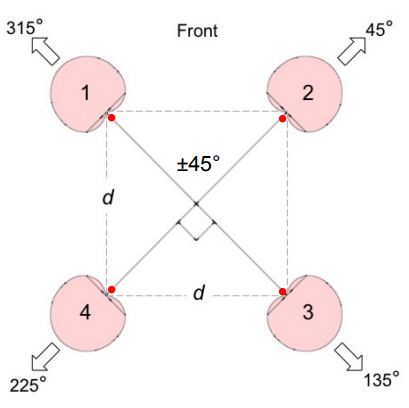
\includegraphics[width = 0.4\linewidth]{images/mic/esma.png}
				\caption{Equal-segment-microphone-array proposed by Michael Williams \cite{esma}}
				\label{esmaSchematic}
			\end{center}
			\end{figure}
			The ESMA was designed to capture sound from 360\textdegree{} in the azimuth plane using four cardioid microphones positioned in a square arrangement, with a distance of 25cm between each capsule. The angles between each microphone should be 90\textdegree{}, creating a stereophonic recording angle (SRA) of $ \pm45 $\textdegree{} \cite{williamsMMAD}, \cite{williams91}. Dr Hyunkook Lee of Huddersfield University found that by changing the distance between each capsule to 50cm, the localisation accuracy of sound sources within a VR environment was improved \cite{esma}. Lee also proposed that an additional four upward-facing cardioid microphones could be added to the array to capture the diffuse sound within the recording environment. The four upward-facing microphones should also have a distance of 50cm between them and are represented by the red dots in Fig. \ref{esmaSchematic}. Inter-channel cross talk is minimised due to the use of spacing and cardioid polar patterns.\\

		\subsubsection{ORTF-3D Surround}

			\begin{figure}[h!]
			\begin{center}
				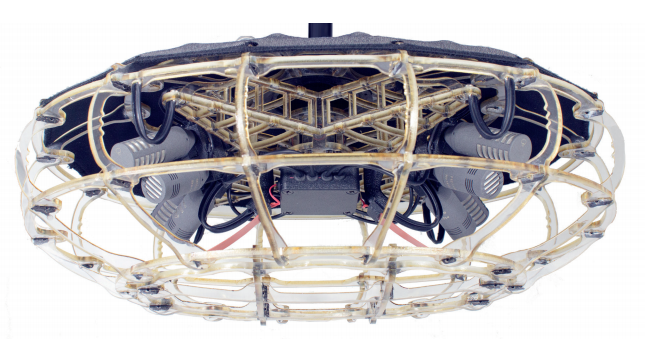
\includegraphics[width = 0.45\linewidth]{images/mic/ortf3D.PNG}
				\caption{ORTF-3D Surround microphone array \cite{ORTF3D2}}
				\label{ORTF3D}
			\end{center}
			\end{figure}

			The ORTF-3D surround is a near-coincident microphone array designed by G\"{u}nther Theile and Helmut Wittek for Schoeps Mikrofone. The bottom plane consists of four supercardioid CCM 41 Schoeps microphones positioned in a 10cm x 20cm rectangle. The capsules are directed to the left front (LF), right front (RF), rear left (LS) and rear right (LR). The angles between the left and right capsules are 80\textdegree{} and 100\textdegree{} between the front and rear capsules. The upper plane consists of four supercardioid CCM 41V Schoeps microphones with the capsules facing upwards (LFh, RFh, LSh and RSh) to create coincident X-Y pairs at 90\textdegree{} between the upper and lower planes \cite{ORTF3D2}. Supercardioid microphones coupled with the spacing between microphones prevent unwanted inter-channel cross talk and comb-filtering effects as well as improved spatial resolution.

		\subsubsection{OCT-9 Surround}
			\label{sec:OCT9}	

			\begin{figure}[h!]
			\begin{center}
				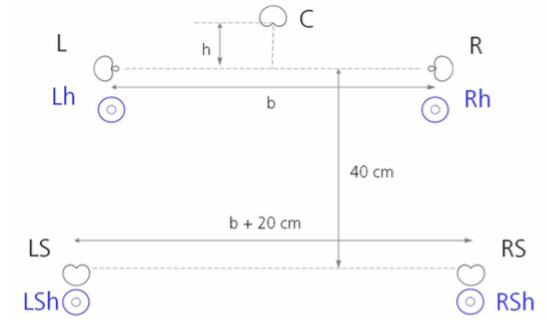
\includegraphics[width = 0.6\linewidth]{images/mic/OCT.png}
				\caption{OCT-9 Surround microphone array \cite{TheileWittek}}
				\label{oct}
			\end{center}
			\end{figure}

			 The OCT-9 Surround microphone array was also designed by G\"{u}nther Theile and Helmut Wittek for the Auro-3D (9.1) loudspeaker arrangement. The front facing section is based on Theile's optimised cardioid triangle surround (OCT-Surround) array, which is used to capture sound for 5.1 multichannel systems \cite{TheileWittek}, \cite{Theile}. This includes four upwards facing supercardioid microphones for diffuse field capture. Each channel should be fed directly to its corresponding loudspeaker in the Auro-3D loudspeaker system.

		\subsubsection{Perspective Control Microphone Array (PCMA)}

			\begin{figure}[h!]
			\begin{center}
				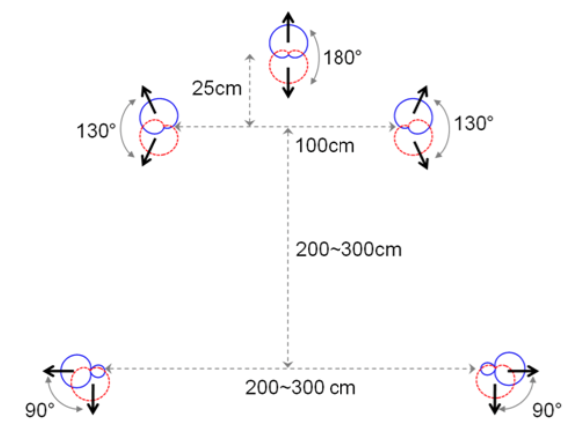
\includegraphics[width = 0.5\linewidth]{images/mic/pcma.png}
				\caption{PCMA arrangement \cite{leePCMA}}
				\label{pcma}
			\end{center}
			\end{figure}
			The PCMA arrangement is similar to OCT-Surround but five widely spaced coincident pairs are used in place of single microphones. Each pair uses cardioid microphones creating virtual microphones through different mixing ratios \cite{leePCMA}. This allows perceived source distance and source width to be changed post-recording \cite{leePCMA}.

		\subsubsection{Hamasaki Cube}

			\begin{figure}[h!]
			\begin{center}
				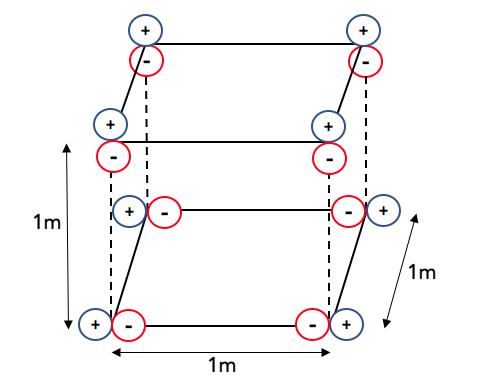
\includegraphics[width = 0.5\linewidth]{images/mic/Hamasaki1.png}
				\caption{Hamasaki Cube Microphone Array}
				\label{ham}
			\end{center}
			\end{figure}

			The Hamasaki Cube microphone array is specifically designed to capture the reverberation and diffuse sound in performance spaces such as concert halls. The array consists of eight bi-directional microphones positioned in a cube arrangement with equal spacing of 1 metre between each microphone. The nulls of each microphone are pointed inwards, which helps to reduce the capture of direct sound. This array is usually used in combination with other direct sound capture arrays to reproduce the full spatial impression of the performance space \cite{TheileWittek}.

		\subsubsection{IRT Cross}

			\begin{figure}[h!]
			\begin{center}
				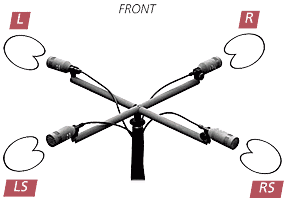
\includegraphics[width = 0.5\linewidth]{images/mic/irt.png}
				\caption{Schoeps IRT Cross microphone array \cite{IRTschoeps}}
				\label{irt}
			\end{center}
			\end{figure}

			The IRT cross array, also known as the 'atmo-cross' is used to capture reflected diffuse sound and direct environmental sounds such as applause and crowd noise\cite{IRTschoeps}. It can be created using four cardioid microphones positioned in a square with 20cm - 25cm spacing between each capsule. The capsules should be facing towards the front left (FL), front right (FR), rear left (LS) and rear right (RS).







% =========----------	[ Space left here for distraction free mode] ----------==========%










\section{Recording at Abbey Road Studios}
	% - Description of recording process
	% - Band + song
	% - List of microphones arrays + positions

	The following section describes the planning process and recording session of this project. All microphones arrays used in the recording session are listed and described including their position within the room. 

	\subsection{Planning}
		% The Band - 5 piece indie rock band that can be spread out across the room
		To produce a VR experience of a live musical performance an appropriate musical ensemble was required. There were a few prerequisites before deciding upon an ensemble, such as deciding upon a musical genre. The style of music needed to be appropriate for a wider demographic and could not be explicit in its nature. The ensemble must also be well-rehearsed and employ a sense of professionalism to ensure that the time available in the studio was used efficiently and productively. With these conditions in place, a London-based Indie-Pop ensemble called 'Nova Neon' were contacted. Nova Neon are a five-piece band who play a sophisticated style of Indie-Pop using a mix of both anechoic sounds and acoustic instruments. The song chosen for the performance was called 'Close Your Eyes' from their album 'Chroma'. This song was chosen for the hard panned left and right guitars which could be exaggerated within an Higher-Order Ambisonic reproduction. \\

		% The room - Studio 3 is large enough to house the band and has heigh ceilings

		The recording location of choice was Studio Three at Abbey Road Studios. The room is large enough to comfortably house the 5 piece band and boasts heigh ceilings that allow for a more diffuse sound-field to exist higher in the room which could be taken advantage of in exploring capturing the ambience of the space using dedicated multichannel microphone arrays.\\


	\subsection{Microphone and Camera Set Up}

		As this research is currently of interest amongst audio engineers and professionals in the audio industry, it was decided to invite other collaborators to participate in the research. Dr Hyunkook Lee from Huddersfield University was invited to attend the recording session to set-up the Equal Segment Microphone Array, which he had shown to perform well at capturing audio for VR. The technical director of Schoeps Mikrofone Helmut Wittek was also contacted with an invitation to collaborate. Schoeps agreed to contribute by supplying their ORTF-3D Surround and OCT-9 Surround multichannel microphone arrays (MMAs). By collaborating with Schoeps Mikrofone and Dr Hyunkook Lee, the research was expanded to include a wider selection of multichannel microphone arrays for subjective analysis. 

		% Floor Plan
		The floor plan for studio three can be seen in Figure~\ref{FloorPlan} annotated with three letters, A (green), B (red) and C (blue) showing the different positions that the Ambisonic microphones, multichannel microphone arrays and 360\textdegree{} video cameras were placed. \\

		% Musician Placement


		 The following sections list the microphones that were placed in each of these positions.

		\begin{figure}
			\begin{center}
				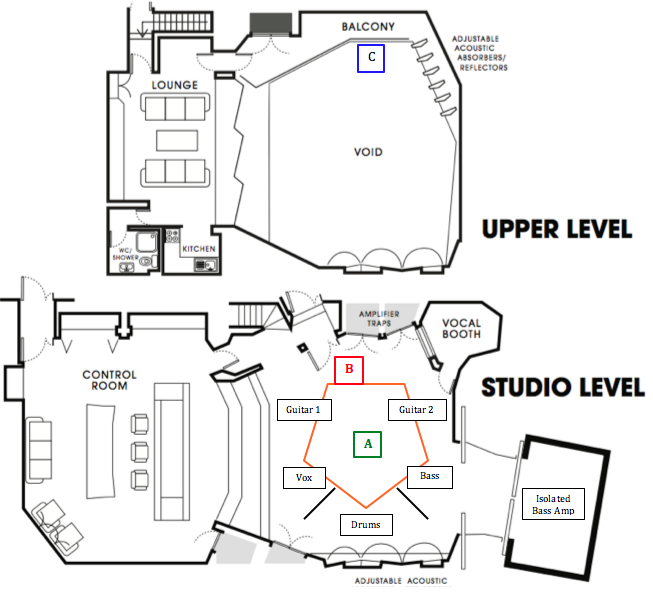
\includegraphics[width = 0.8\linewidth]{images/other/FloorPlan.png}
				\caption{Preliminary floor plan of the recording session in Studio Three \cite{Studio3}}
				\label{FloorPlan}
			\end{center}
		\end{figure}

		% List of all microphones + Cameras

		% Position A
		\subsubsection{Position A}

			Position A is located in the centre of recording space and in the middle of the musicians. This is where the visuals for the VR experience were captured in 360\textdegree{} using the GoPro Omnirig. The Soundfield ST450 MKII, EM32 Eigenmike, Equal-Segment-Microphone-Array (ESMA) and Schoeps ORTF3D Surround were also set-up in this position to capture direct sound radiating from the instruments.\\

			\paragraph{GoPro Omnirig}
			The GoPro Omnirig is a synchronised six-camera array used to capture 360\textdegree{} videos \cite{gopro}. It was placed at position A at a height of 160cm to the bottom of the array. GoPro number one in the Omnirig was positioned to face a reference point at the back wall where the drum kit would be set-up.\\

			\paragraph{Neumann KU100}
			The KU100 was positioned to be facing towards the reference point (drum kit). Though this would not be used in the listening tests  it was included so it could be used to compare against the other recording techniques.\\

			\paragraph{EM32 Eigenmike}
			The Eigenmike was placed on its side just above the GoPro Omnirig at a height of 1.81m shown in figure~\ref{STApos}. The aim was for the Eigenmike to capture the direct sound from the instruments and provide a soundfield recording 'canvas' on which the spot microphone recordings could be placed within a Higher-Order Ambisonic framework. \\

			\paragraph{Soundfield ST450 MKII}
			The soundfield microphone was placed at a height of 2m and placed on its side above the GoPro Omnirig and Eigenmike. It is worth noting that the 'end fire' switch must be activated on the ST450 pre-amplifier if the microphone is placed on its side for recording. The 'end fire' setting adjusts the X, Y and Z axis data to ensure that the correct soundfield orientation is captured.\\

			\begin{figure}[ht]
			\begin{center}
				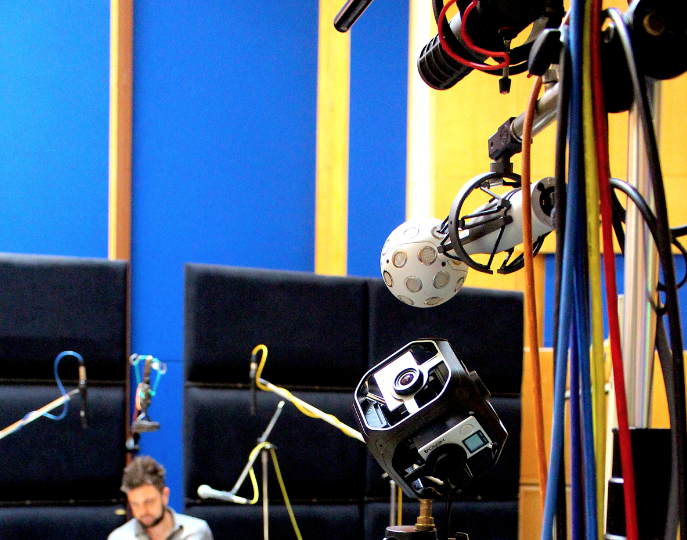
\includegraphics[width = \linewidth]{images/other/ST450pos.png}
				\caption{Placement of the first Soundfield ST450 MKII microphone, Eigenmike and GoPro Omnirig at position A}
				\label{STApos}
			\end{center}
			\end{figure}

			\paragraph{Equal Segment Microphone Array (ESMA)}
			The ESMA is based on the 'four segment array' proposed by Michael Williams in 1991 \cite{williamsMMAD}, \cite{williams91}. It was designed to capture sound from 360\textdegree{} in the azimuth plane using four cardioid microphones positioned in a square arrangement, with a distance of 25cm between each capsule. The angles between each microphone should be 90\textdegree, creating a stereophonic recording angle (SRA) of $ \pm45 $\textdegree \cite{williamsMMAD}, \cite{williams91}. 

			Through listening tests, Dr Hyunkook Lee of Huddersfield University found that by changing the distance between each capsule to 50cm, the localisation accuracy of sound sources within a VR environment was improved \cite{esma}. Each of the four microphones on the azimuth plane were angled down by 45\textdegree{} to face the instruments and optimise direct sound capture from the instruments. The array was positioned at a height of 2.15m, with the upward facing microphone capsules reaching a height of 2.28m. The four additional upward-facing cardioid microphones were added to capture some of the diffuse sound within the recording environment. The four upward-facing microphones were also set-up with distance of 50cm between each capsule. The use of cardioid microphones and the wide spacing between each microphone capsule helps to minimise inter-channel cross-talk, whilst still providing satisfactory localisation of sound sources within the azimuth plane.\\


			\paragraph{ORTF-3D Surround}
			The supercardioid microphones used in this array allow for sufficient signal separation between each microphone to avoid unwanted inter-channel cross-talk and comb-filtering effects. The spacing between each microphone follows the principles of the ORTF technique to allow for the required inter-channel time differences and improved spatial resolution to be included into the recording. The ESMA and ORTF can both be seen at position A in figure~\ref{esma}.\\


			\begin{figure}[h]
			\begin{center}
				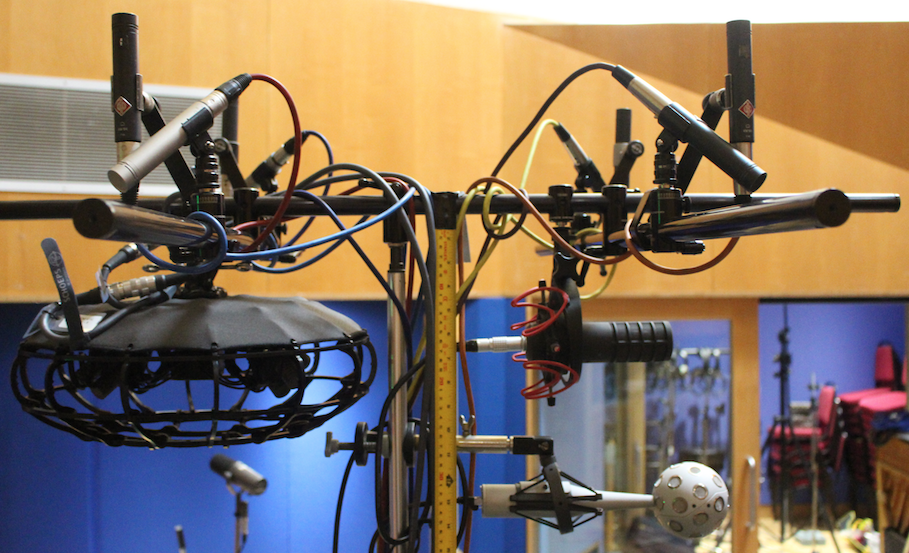
\includegraphics[width = \linewidth]{images/other/esmapic.PNG}
				\caption{Picture of the ORTF-3D Surround Array without windshield (top) and the ESMA (left) just underneath. The front of the arrays was positioned facing the reference point at the drum kit.}
				\label{esma}
			\end{center}
			\end{figure}

		% Position B
		\subsubsection{Position B}
			Position B is located to the rear of Studio Three near the entrance. The objective for this position was to capture a 180\textdegree{} view of the musicians and provide a different audio and visual perspective for the VR experience. The Samsung Gear 360 camera, Stereo X-Y pair, OCT-9 Surround, Perceptual Control Microphone Array (PCMA) and Sennheiser AMBEO Ambisonic microphone were placed at position B to capture both audio and video from this viewing (and listening) position.\\

			\paragraph{Samsung Gear 360}
			The Samsung 360 was used to provide a 180\textdegree{} visual perspective of the live performance with the musicians in front of the viewing position. The camera, multichannel microphone arrays and Ambisonic microphones were directed at the same reference point facing towards the drum kit. \\

			\paragraph{Stereo X-Y Pair}
			A coincident stereo X-Y microphone arrangement was set-up at position B as a reference. Two Neumann KM184 cardioid microphones were arranged to produce a stereo recording angle of 115\textdegree{} and positioned to face the drum kit at a height of 1.94m to the coincident point.\\

			\paragraph{Sennheiser AMBEO}
			The Sennheiser AMBEO is a B-format Ambisonic microphone similar to the Soundfield ST450 MKII. It is also capable of recording First-Order Ambisonics using a tetrahedral coincident arrangement of four cardioid microphone capsules \cite{ambeo}. The AMBEO is available to purchase at a considerably lower price compared to the Soundfield ST450 MKII and therefore it would be of interest to compare their performance. The AMBEO was placed at position B, just above the Samsung Gear 360 camera at a height of 1.59m to the centre of the microphone grill. The positioning of the AMBEO did cause some occlusion where the Samsung camera was obstructing sound from entering the bottom of the microphone, shown in figure~\ref{ambeopic}. This was not ideal but due to limited space available the positioning was deemed appropriate. \\
			
			\begin{figure}[h]
			\begin{center}
				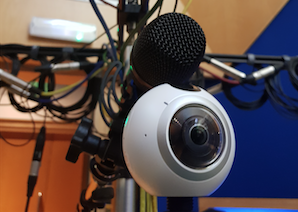
\includegraphics[width = \linewidth]{images/other/ambeopic.png}
				\caption{Placement of the Sennheiser AMBEO and Samsung Gear 360 camera at position B}
				\label{ambeopic}
			\end{center}
			\end{figure}

			\paragraph{Perspective Control Microphone Array (PCMA)}
			Due to space and equipment limitations encountered during the recording session, the PCMA set-up used the front-centre, rear-facing and upward-facing microphones from the OCT-9 Surround. Coincident stereo pairs were set-up for only the front left and front right positions. The PCMA was set-up at a height of 1.82m to the microphone capsules.\\

			\paragraph{OCT-9 Surround}
			The OCT-9 Surround microphone array was designed by G\"{u}nther Theile and Helmut Wittek for the Auro-3D (9.1) loudspeaker arrangement. The front facing section is based on Theile's optimised cardioid triangle surround (OCT-Surround) array, which is used to capture sound for 5.1 multichannel systems \cite{TheileWittek}, \cite{Theile}. Four upward-facing supercardioid microphones are added to the OCT-surround to create the complete OCT-9 Surround array. Using directional microphones in this way again helps to increase channel separation and avoid unwanted inter-channel cross-talk. The front three microphones are used to capture direct sound whilst the rear and upward-facing microphones capture the diffuse sound and ambience of the recording environment. \\



		% Position C
		\subsubsection{Position C}
			Position C was located behind position A at the rear of Studio Three. At position C, the IRT Cross, Hamasaki Cube and second Soundfield ST450 MKII microphone were placed much higher in the room in contrast to the multichannel microphone arrays located at positions B and C. The aim was for the height arrays and Ambisonic microphone in position C to record more of the diffuse sound existing higher up in the room and capture the ambience of the recording space.\\

			\paragraph{IRT Cross}
			The IRT cross or 'atmo-cross' is a multichannel microphone array generally used to capture diffuse sound and direct environmental sounds such as applause and crowd noise. It can be created using four cardioid microphones positioned in a square with 20cm - 25cm spacing between each capsule \cite{IRTschoeps}. The IRT Cross can also be used in combination with other arrays to allow for the capture of both direct and diffuse sound to provide a full spatial representation of a musical performance within an environment. The IRT Cross was positioned at a height of 3.5m at position C, which helped to reduce direct sound capture and increase the diffuse sound captured.\\


			\paragraph{Hamasaki Cube}
			The Hamasaki Cube is a multichannel microphone array specifically designed to capture the reverberation and diffuse sound in performance spaces such as concert halls. Due to space limitations, the dimensions of the Hamasaki Cube were reduced from 1m to 0.7m. Eight Neumann U87 condenser microphones were used to create the Hamasaki Cube, which was positioned at a height of 3m to the microphone capsules on the lower layer of the cube. The microphone capsules on the upper layer of the Hamasaki Cube reached a total height of 3.7m. Given the widely spaced microphone arrangement and the height of the Hamsaki Cube creating sufficient inter-channel time and level differences, it was expected to perform well at capturing the ambience Studio Three.\\

			\paragraph{Soundfield ST450 MKII}

			The second Soundfield ST450 MKII Ambisonic microphone was positioned between the front two microphones of the IRT Cross at a height of 3.45m to centre of the microphone grill. This allowed for a First-Order Ambisonic soundfield recording higher up in the recording space in the hope of capturing more of the rooms ambience. \\

			All three microphones at position C is illustrated in figure~\ref{pos3} and the separation between position A and C is shown in figure~\ref{AvsC}.\\

			\begin{figure}[h]
			\begin{center}
				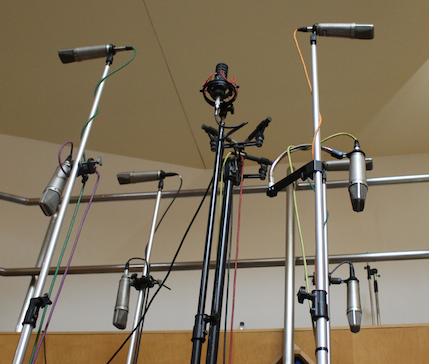
\includegraphics[width = \linewidth]{images/other/positionC.png}
				\caption{Placement of the second Soundfield ST450 MKII, IRT Cross and Hamasaki Cube at position C}
				\label{pos3}
			\end{center}
			\end{figure}

			\begin{figure}[h]
			\begin{center}
				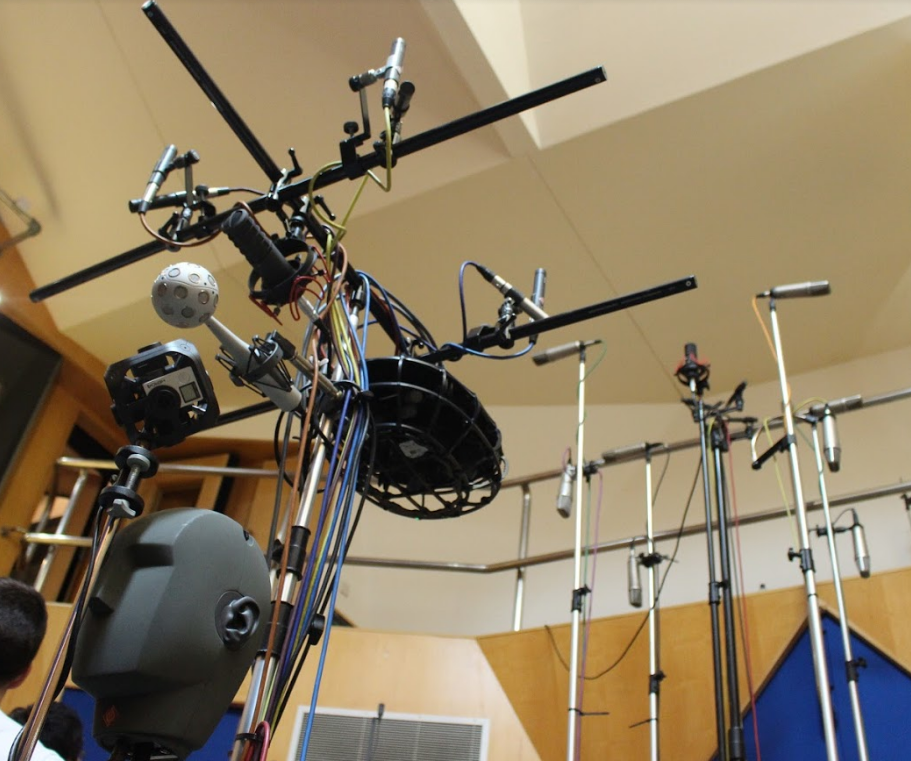
\includegraphics[width =\linewidth]{images/other/posAC.png}
				\caption{Microphones at position A with microphones in position C in the background}
				\label{AvsC}
			\end{center}
			\end{figure}

		\subsubsection{Spot Mics}

			For an ensemble such as this it is natural when performing for each musician to be spot miked due to the natural variation in dynamics. If only the microphone arrays described above were used then the lead and backing vocalists would be drowned out by the drums. As it was also decided that the bass guitar would be recorded in isolation to avoid the lower bass frequencies overpowering other sound sources within the recording space, the bass guitar would not be picked up by the arrays at all. Therefore each instrument required their own spot mic to ensure that the vocals and bass guitar could be mixed in consistently with the rest of the ensemble. The spot microphones were positioned by Abbey Road engineers using their usual recording techniques and work flow. The spot microphones and placement for each instrument are detailed below.\\
			
			\paragraph{Drums}

			Each section of the drum kit was recorded using spot microphones, the details for which are displayed in table~\ref{spots}.\\

			\begin{table}[h]
				\centering
				\resizebox{0.45\textwidth}{!}{%
				\begin{tabular}{m{15mm} lll}
					Section & Microphone Model & Polar Pattern & Position \\
					\hline
					\multirow{2}{*}{Kick Drum} & Shure Beta 52a & Cardioid & Inside the kick drum  \\
					& Neumann U47-fet & Cardioid & In front of the kick drum\\
					\hline
					\multirow{2}{*}{Snare Drum} & Shure Unidyne III 57 & Cardioid & Top of snare drum \\
					& AKG 414 & Cardioid & Underneath snare drum \\
					\hline
					Hi-Hat & Shure SM58 & Cardioid & Above Hi-Hat \\
					\hline
					Knee & Sony C38 & Cardioid & Above drummer's right knee \\
					\hline
					Mid Tom & Beyer M201 & Cardioid & Above mid tom \\
					\hline
					High Tom & Beyer M201 & Cardioid & Above mid tom \\
					\hline
					Mono Overhead & Coles 4038 & Bi-directional & Above the drummers head \\
					\hline
					Stereo Overheads & 2 x DPA 4011 & Cardioid &  Standing position for Vocalist \\
					\hline
					Stereo Drum Room Mics & 2 x DPA 4006 & Omnidirectional & 3 feet in front of the drum kit \\
					\hline
				\end{tabular}}
				\caption{A table of the spot microphones used for recording the ensemble}
				\label{spots}
			\end{table}

			\paragraph{Bass Guitar}
				To prevent excessive low frequency spill from the bass guitar, an Ampeg B15N Portaflex bass amplifier was placed in an isolation booth and recorded with a Neumann FET 57 microphone. As it would look unnatural to hear the bass but see no bass amplifier in the VR experience, a 'dummy' bass amp was placed in the room to the left of the bassist with the rest of the musicians. Figure~\ref{drums} shows the FET mic placement on the dummy amplifier. \\

				\begin{figure}[ht]
				\begin{center}
					\includegraphics[width = \linewidth]{images/other/dummycab.JPG}
					\caption{Neumann FET 57 placement on the 'dummy' amplifier}
					\label{drums}
				\end{center}
				\end{figure}

			\paragraph{Electric Guitars}
				An Orange Crush 60R amplifier and a Fender Blues Junior amplifier were placed on the right and left of the central position with both guitarists respectively. Both amplifiers were placed on chairs to raise the height and angled up to allow a clear path for sound to travel towards the multichannel microphone arrays and Ambisonic microphones. Neumann U87 condenser microphones were also placed centrally in front of the amplifiers. Direct signals were also taken from both guitarists pedal boards. Effort was made to match the volumes of both guitar amplifiers to create a balanced sound within the room which would be captured by the multichannel microphone arrays. Figure~\ref{guitarAmps} shows both of the electric guitar amplifiers as described.\\

				\begin{figure}
					\centering
					\subfloat[][Neumann U87 placement on Guitar 1 amplifier]{
						\includegraphics[width=.5\linewidth]{images/other/gtr1.JPG}
						\label{fig:sub1}}
					\subfloat[][Neumann U87 placement on Guitar 2 amplifier]{
						\includegraphics[width=.5\linewidth]{images/other/gtr2.JPG}
						\label{fig:sub2}}
					\caption{Spot microphones on the electric guitar amplifiers}
					\label{guitarAmps}
				\end{figure}
				

			\paragraph{Vocals}
				The lead vocalist was recorded using a Shure SM7B microphone and positioned to the right of the drum kit, shown in figure~\ref{voxmic}. Acoustic panels were placed between the drums and vocalist to minimise any spill picked up by the vocal microphone. Backing vocals provided by guitarist 2 were also recorded using a Shure SM7B, whilst the drummers backing vocals were recorded using a Shure SM58. Microphone directivity was crucial to reject as much off-axis sound as possible.\\

				\begin{figure}[ht]
				\begin{center}
					\includegraphics[width = \linewidth]{images/other/vox.JPG}
					\caption{Picture showing the placement of the Shure SM7 and acoustic panels}
					\label{voxmic}
				\end{center}
				\end{figure}


	\subsection{Recording Process}
		Once the equipment was set-up for the recording session, each of the microphone channels from each multichannel microphone array and Ambisonic microphone were connected to tie lines in the live room and routed to a channel on the SSLJ 9000J 96-channel mixing console in the control room. The spot microphones used the pre-amplifiers on the mixing console as did each channel of the Hamasaki Cube. For the Ambisonic microphones (Soundfield ST450 and Sennheiser AMBEO), a stepped pre-amplifier was required to ensure that the gain levels set for each of the W, X, Y and Z channels were identical. There were thirty six AMS Neve Montserrat pre-amplifier channels and twelve AMS Neve 1081 pre-amplifier channels available for the session. Care was taken to ensure that each microphone array and Ambisonic microphone used the same pre-amp model for each of their individual channels. 

		The session was recorded on a ProTools HD rig \cite{ProToolsHD} at a sampling rate of 48kHz and a bit-depth of 24. This was the practical option as there were in excess of ninety channels being used and the file sizes had to be taken into consideration. Recording at 48kHz/24bit allowed for high-quality recordings whilst ensuring that the file sizes were still practical to work with in the post-production process. The Eigenmike was recorded onto a separate laptop that was synchronised to the ProTools HD session and time-stamped, allowing for the Eigenmike to be recorded simultaneously with the ProTools HD session.

		A 5.1 surround system comprising of five Bowers and Wilkins 800D speakers was used for monitoring in the control room. Where possible, the arrays were 'folded down' to the 5.1 system for monitoring. The spot microphones were monitored in stereo as would be the case in a conventional recording session. Although the monitoring system did not allow for 3-D audio reproduction, it was useful to listen and switch between each of the different channels and different microphone arrays in real-time. Timbral qualities such as the brightness of the microphones could be identified whilst monitoring and it provided an early indication to how each of the different multichannel microphone arrays and Ambisonics microphones might sound after the implementation stage.

		%\section{Recording Summary}

		%Including the Eigenmike there were 122 channels that needed to be recorded simultaneously in the session for each performance. A session of this size required meticulous planning and attention to detail to ensure everything was set-up, documented, routed and recorded successfully. Due to the size of the session, no one person was in a position to have a clear overview of the whole recording process. For each take the cameras needed to be checked and set to record, the band needed to be given feedback and each input channel had to be monitored to ensure that everything was being recorded as planned. Only as a team was it possible to undertake such an intensive audio and visual recording session in one day.







% =========----------	[ Space left here for distraction free mode] ----------==========%










\section{Post-Processing and Workflow Set Up} % Think of a better heading

	Once the recording at Abbey Road Studios was complete, the recording session was assessed using 5.1 surround sound system with a PC running ProTools 12 in the media suit at the University of York. In a normal audio editing situation the best bits of every take could be split and merged together. However as this would cause discontinuity in the video and the audio, coupled with the impracticality imposed by the abundance of audio tracks, a single take must be used. It was decided that take eight of 'Close Your Eyes' would be used as the track for testing. This take was exported and condensed into a smaller project where each track was exported as a WAV file ready to be imported into Reaper for Ambisonic processing.

% Once each audio track had been previewed, the next objective was to decide on the best take recorded during the session. Each take contained minor instrumental issues such as wrong notes and timing issues.

	\subsection{Video Post-Production}
		Before the audio could be mixed within an Ambisonic framework, the 360\textdegree~videos needed to be produced. This was to ensure that the sound sources were accurately aligned with the visual in the VR environment, i.e the audio of the lead vocals needed to sound as though they were coming from the lead vocals. As two different 360\textdegree cameras were used during recording, two different methods of spherical video production were used.

			\subsubsection{Video Stitching and Editing}

				\paragraph{Position A - 360\textdegree~perspective GoPro Omni}
					The GoPro Omni rig comes paired with a software suite including Omni Importer that can be used for easily importing 6 individual video files that can then be stitched together and edited to create a spherical video ready for use in a VR workflow using Kolor's AutoPano Video software. The videos files from the six GoPro cameras for take eight were imported using the Omni Importer software and stitched together in AutoPano Video. With time and experience it is possible to optimise the video stitching process to prevent the 'ghosting' effect in which subjects/objects placed too close to the GoPro Omni rig are distorted as they are split between two of the GoPro cameras and part of the subject/object is lost within a blind spot. It can be seen in the video that the guitarist have fallen victim to such an effect.\\

					Once stitched together the video was exported as an mp4 file and imported into Adobe Premiere Pro \cite{AdobePremiere} for further editing. The colour balance was adjusted to add some vibrancy to the visuals, before a title was added at the beginning of the video. Fades were also applied at the beginning and end of the video to stop the video starting and ending abruptly. The editing process in Adobe Premiere was simple but necessary to produce a video suitable for use in the VR experience and listening tests.

				\paragraph{Position B - 180\textdegree~ perspective Samsung 360}
					Videos shot using the Samsung 360 camera can be stitched and processed using Samsungs dedicated software 'Gear 360 Action Developer'\cite{actiondev}. As the camera only uses two fish eye lenses it is not possible to adjust where the software stitches the two videos together meaning that any ghosting effect that occurs can not be removed. As the Samsung 360 was placed further away from the musicians and the front facing lens was directed towards the entire ensemble, ghosting did not affect any subjects of interest. Once the video was stitched the same post-processing in Adobe Premiere was applied to the video.\\
			
			\subsubsection{Video Playback and Head-Tracking}
				 Kolor's GoPro VR Player \cite{GoProVR} can be used to open and preview 360 videos with built in head-mounted display (HMD) support allowing the video to be navigated using either the HMD's motion sensors or by clicking on the video and dragging. In the case of this project an Oculus Development Kit 2 (DK2) \cite{OculusDK2} headset was utilised. Using an external piece of software it is possible to send the head-tracking data from GoPro VR Player to Reaper to synchronise the soundfield rotation required for head movement. This is explained in section ~\ref{spooks}.


		\subsection{Audio Post-Production}
			
			\subsubsection{Creating a Higher-Order Ambisonics Template in Reaper}

				Reaper \cite{Reaper} is (at the time of writing) currently the only DAW that allows for up to 64 channels per track making it perfect for Higher Order Ambisonic (HOA) production. A Reaper template utilising a 36 channel bus for each of the microphone arrays was produced, allowing the microphone arrays to be encoded up to Fifth-Order Ambisonics. Each of the 36 channel buses for each of the microphones arrays were then routed to a 36 channel track containing a sound field rotator and Fifth-Order binaural decoder.
				
				The Eigenmike was imported and processed on its own 36 channel track and routed to a sound field rotator and 3\su{rd} decoder. As the Eigenmike was placed on its side during the recording session, the orientation was corrected by applying an additional sound field rotation.

				The B-Format recordings produced by the Soundfield ST450 MKII microphones created four tracks for each of the W, X, Y and Z information channels. The separate W, X, Y and Z channels were assigned to a four channel 'parent' track in Reaper. The Soundfield ST450's also required their own 4 channel First-Order Ambisonic tracks and decoders.\\

				Once the template was produced, the raw audio files were imported and grouped into the appropriate microphone groups. The following sections describe the processing of the raw audio files to produce a Fifth-Order head-tracking binaural mix. \\

			\subsubsection{Treatment and Ambisonic Encoding}
				Before anything was encoded into an Ambisonic format, Reaper 'ReaEQ' equalisation plugins were applied to each of the microphone tracks. It is important to EQ the tracks before Ambisonic encoding to prevent spherical harmonic distortion. In some instances where the microphones were placed close to the instruments, subtle filtering was applied such as a 6db reduction below 110Hz on the drum kit to reduce the overpowering bass drum in an attempt to increase the clarity of the mix. Individual microphone channels within an array were treated with the same equalisation to provide consistency for the listening tests. The spot microphones were treated by Mirek Stiles from Abbey Road Studio before being imported into the Reaper project. This was to ensure that the spot microphone recordings were of good tonal quality as a standard mix should be. \\

				Inserted in the FX chain next was a Fifth-Order AmbiX encoder. The AmbiX encoders use the ambiX Ambisonic format, with the Ambisonic Channel Number (ACN) ordering and SN3D normalisation conventions \cite{AmbixFORMAT}. The AmbiX encoder plug-ins provide a graphical interface from which one can position mono or stereo sound sources to specific azimuth and elevation angles around the VR environment, shown in figure~\ref{ambixEncode}.

				% Spot mics
				The spot microphones were duplicated and split into two groups. The first group was used to encode the spot microphones relative to the video from viewing position A and the second for viewing position B. This was done by opening the video in GoPro VR Player and setting the view to the reference 0\textdegree~position, in this case the centre of the drum kit. The individual spot microphones were then placed in the 3-dimensional space using the ambiX encoder plug-ins and using the Oculus DK2 as a visual reference. A B-Format impulse response of St Albans Cathedral \cite{OpenAir} was obtained from the OpenAir online impulse response library to create a convolution reverb effect on the lead and backing vocals. Using the AmbiX MCFX Convolver4 plug-in \cite{AmbixPLUGINS}, \cite{AmbixDOWNLOAD} inserted onto 4-channel auxiliary track, it was possible to achieve a 3-D reverb effect that suited the VR experience better than a standard mono or stereo reverb effect. The vocal tracks could then be sent individually to the B-Format reverb bus to achieve the required wet/dry ratio.

				% Microphone Arrays
				Each microphone arrays was encoded in the same way that they should naturally be listened to. For example, the OCT surround channels were encoded in the same position that the speakers are designed to be placed as described in section~\ref{sec:OCT}. For other microphones arrays that are not designed to be fed straight to a specific speaker layout, each microphone channel was encoded into a position relative to the listener as the microphones were placed in the room.

				\begin{figure}[h]
				\begin{center}
					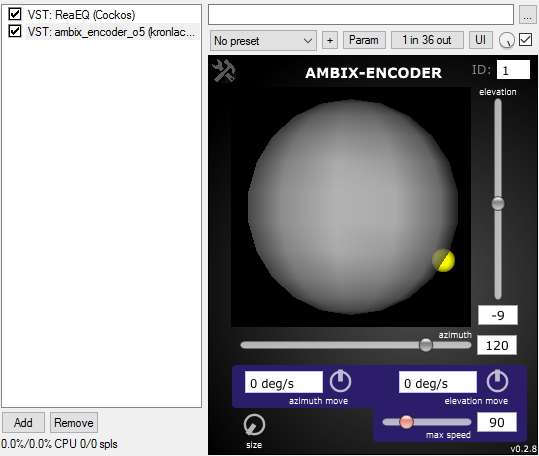
\includegraphics[width = \linewidth]{images/other/ambix.png}
					\caption{Screenshot of the Fifth-Order AmbiX encoder for a mono sound source (Kick Drum)}
					\label{ambixEncode}
				\end{center}
				\end{figure}

				% ST450
				For the raw SoundField ST450 recordings it was necessary to convert the Soundfield's B-Format recordings from the Furse-Malham format to the ambiX format using the AmbiX Converter plug-in \cite{AmbixPLUGINS}, \cite{AmbixDOWNLOAD}, which corrected the channel sequence and normalisation before the decoding stage. Apart from the format conversion, no other Ambisonic encoding was required as the Soundfield ST450 MKII microphone captured the full spherical soundfield with sound sources already in the correct locations. 

				% Eigen
				Before importing into the reaper project, the Eigenmike recording was encoded into Third-Order Ambisonics using the EigenUnits plug-in by mh acoustics \cite{eigen}. This then meant the 36 channel 3\su{rd} order Eigenmike tack could be imported into the Reaper project without he need to encode the track in real time. As the Eigenmike was mounted on its side during the recording session, the soundfield had to be rotated by -90\textdegree{} in the elevation plane to compensate for this positioning using an AmbiX Third-Order Rotator \cite{AmbixPLUGINS}.

			\subsubsection{Binaural Decoding}

				Each of the microphone array channels and spot mics were routed to a final mixing bus used for 5\su{th} order decoding. The Egienmike and Soundfield microphones were sent to a 3\su{rd} order and 1\su{st} order mix bus respectively. An ambiX Binaural Decoder plugin was inserted onto each of the mix buses. The plug-in requires a configuration files that contains information regarding where the HRTF data set to use is stored, the virtual loudspeaker layout that should be used and provides a decode matrix to multiple the signal vector by \cite{Girafe}. Configuration files for the following Ambisonic orders and speaker layouts were taken from the SADIE database \cite{SADIE}:

				\begin{center}
				%\resizebox{0.45\textwidth}{!}
				\end{center}


				As Google have recently adopted the KU100 measurements from the SADIE database to use in their YouTube360 \cite{youtube360} online platform, the same HRTF data set was used in the binaural decoding process. The HRTF set first needed to be converted from 44.1kHz/16-bit as downloaded from the SADIE database to 48kHz/24-bit to match the settings of the Reaper project using the r8brain V1.9 \cite{r8brain} application.

		\subsection{Audio Visual Synchronisation}

			When turning your head in the real world, sound sources remain static in 3D space and your perspective of the world is rotated both visually and sonically. When listening to a binaural decode over headphones however, when you turn you head the headphones and the audio being played through them stay in place on your head. If something was encoded you sound like it was coming from your right, it would sound like it was coming from your right no matter where you turned your head. To create a truly immersive audio visual environment the sound field must be rotated as the visuals are. 

			This can be achieved by using a sound field rotation plug-in and feeding it real time rotation data. 

			SpookSyncVR \cite{SpookSync} is built in Max MSP as a stand-alone application that allows data exchange between GoPro VR Player and Reaper using Open Sound Control (OSC). Using SpookSyncVR it is possible to gather the X (yaw) and Y (pitch) positional data from the headset and transfer the information to Reaper so that the sound field can be rotated accordingly. For this an Ambix Rotator plug-in was inserted into each of the three decoder tracks just before the binaural decoding plug-in for which the yaw and pitch data from GoPro VR Player were assigned to control the values of the yaw and pitch data of the rotator plug-ins. By designating the GoPro VR Player as the 'master' and Reaper as the 'slave' it was possible to synchronise, play and stop the audio and video together. 
	
		

\section{Listening Tests}
	% Describe the listening test process

	Two rounds of listening tests were conducted for viewing position A (test 1) and B (test 2). The procedure was identical however the data used, such as video and microphone configurations used were different for each. Participants were recruited from the University of York and Abbey Road Studios for both tests, all of who were required to have some previous experience with mixing/producing and/or spatial audio. The number of participants recruited for each test were as follows:

	\vspace{5pt}
	\begin{tabular}{l c c c}
		& UoY & Abbey Road & Total\\ 
		Test 1 & 15 & 4 & 19\\ 
		Test 2 & 29 & 9 & 38\\ 
	\end{tabular}

	\subsection{Attributes Focus Group}
		The aim of the listening test was to assess the performance of each microphone array configuration for a VR environment in terms of its spatial and timbral quality. Due to the subjectivity of such a test, a focus group was assembled with the purpose of producing a list of mutually agreeable adjectives to use to describe certain spatial and timbral attributes. The attributes chosen to use within the listening tests are shown in table\ref{table:attTable}. \\

		% Table of Spatial and Timbral attributes
		\begin{table}[h]
			\begin{tabular}{m{2.2cm} | m{0.31\textwidth}}
				\textbf{Attribute} & \textbf{Description} \\ \hline
				\multicolumn{2}{l}{\textbf{Spatial}} \\ \hline
				Locatedness & How easily you can locate a sound source within the VR environment \\
				Sense of Space & How well the space where the recording was made is perceived \\
				Externalisation & Perception of sound coming from all around your head \\
				Envelopment & Whether the sounds are perceived to originate inside of outside of the head \\ \hline
				\multicolumn{2}{l}{\textbf{Timbral}} \\ \hline
				Full & Abundance of low frequencies present \\
				Bright & Abundance of high frequencies present \\
				Flat & Lack of high and low frequencies present \\
				Rich & The mix sounds good with both high and low frequencies \\
				Realistic & The sounds heard in the VR experience are realistic (sound like real instruments) and timbral characteristics have been preserved. \\
				Loud & The perceived level sounds high
			\end{tabular}
			\caption{Table of Spatial and Timbral Attributes}
			\label{table:attTable}
		\end{table} 
			

	\subsection{Procedure}

		Using an Oculus DK2 headset and a pair of Audio Technica MH50x headphones, participants were presented with an 80 second VR sample of the recording session which included the songs intro, verse and chorus using one of the microphone arrays appropriate for the samples viewing position. Once the clip was finished participants would answer a questionnaire that was spit into two main sections. The first asked them to rate on a scale of 1 - 10 each of the spatial audio attributes listed in table \ref{table:attTable} where 1 indicated they did not experience that particular attribute well and 10 being that they experience that attribute very well. The second section asked them to select as many of the timbral attributes they felt best described the overall timbre of the clip. Participants were also asked to rate on a scale of 1 - 10 how much they enjoyed the VR experience. This procedure was repeated a number of times depending on the number of microphone arrays to be presented (8 times for test 1 and 7 times for test 2). The order in which samples were presented was randomised per participant.

		To ensure a uniform understanding of the list of attributes that were used in the questionnaire a short training exercise was conducted before each test. This involved taking the participants through each of the attributes with audio examples. 









% =========----------	[ Space left here for distraction free mode] ----------==========%










\section{Analysis Overview}

	All test data was recorded using a Google Form and collated into a large document upon finishing the testing period. All data was then imported into MATLAB for analysis. Table~\ref{image:results_sum} shows the average spatial attribute results for each microphone across each spatial attribute. The highest scores are highlighted in green. The directional OCT microphone array from microphone position and viewing position B scored highest for 'Locatedness' and scored the highest along with the Hamasaki Cube, a diffuse-field microphone array located at position C for 'Sense of Space'. The Hamasaki Cube when viewing from position A scored the highest for 'Externalisation' and 'Envelopment' which results in the highest over all spatial attribute average score. A break down of timbral attribute scores is covered in section~\ref{ana4}\\


	The following six sections will be used to further break down and analyse the data: \\

	\begin{tabular}{r p{5.5cm}}
		Analysis 1: & Does viewing position affect Spatial Attribute rating? \\
		Analysis 2: & Does the choice of microphone array affect Spatial Attribute score? \\
		Analysis 3: & What is the effect of using Directional or Diffuse-Field Arrays? \\ 
		Analysis 4: & Does perception of timbre change with difference viewing positions? \\
		Analysis 5: & Is there a correlation between spatial attribute score and selected timral attributes? \\
		Analysis 6: & Is there a correlation between the enjoyment rating and spatial audio attributes?
	\end{tabular}
	
	\begin{table}
	\begin{center}
		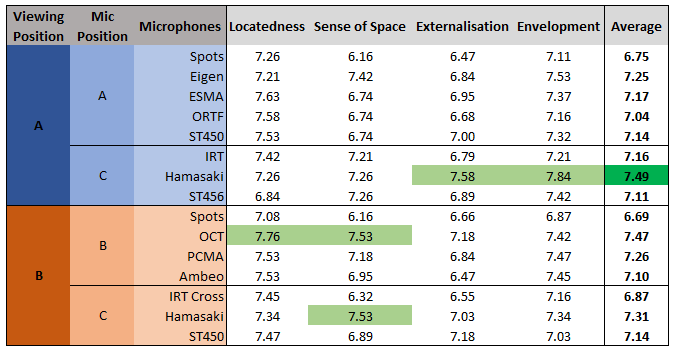
\includegraphics[width=0.45\textwidth]{images/graphs/results_sum_graph_V3.PNG}
		\caption{Table containing the average spatial attribute scores for all microphone with on over all average spatial attribute score. Highest scoring microphones are highlighted in green.}
		\label{image:results_sum} 
	\end{center}
	\end{table}	

	This will be followed by an summary section with conclusions draw from each analysis section.

	






% =========----------	[ Space left here for distraction free mode] ----------==========%









\subsection{Analysis 1: Does viewing position effect spatial attribute scores?}
	\label{ana1}

		% Ana1 Intro
		To assess the potential effect of viewing position on spatial attribute score, data was grouped into 8 sections: An average score for each spatial audio attribute (4 groups) each split into the average score for viewing position A and B (8 groups) illustrated in figure \ref{image:AvsB}. \\

		\begin{figure}
			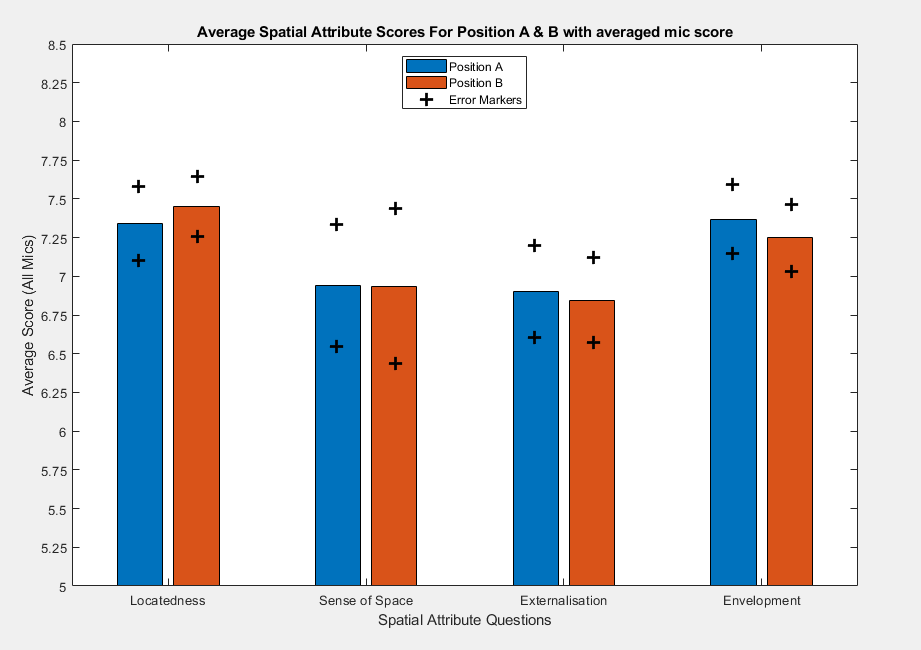
\includegraphics[width=0.5\textwidth]{images/plots/AvB_Bar_error.PNG}
			\caption{Bar chart showing average spatial attribute score for each spatial attribute at viewing position A and B}
			\label{image:AvsB} 
		\end{figure}

		It can be seen that the average spatial attribute score for viewing position A and B for each spatial attribute are close with the difference in overall mean score being 0.02. Running a Two-Sample T-Test between each of the four spatial attribute groups (e.g A vs B for locatedness etc) indicates no statistical significance. Running the same test for the averaged combined spatial attribute score (average of all four spatial attribute scores) also indicates no statistical significant between viewing position. This is made clear in figure \ref{image:AvsB_dist} illustrating the overall similarity in the distribution of scores for viewing position A and B. \\
		
		% NOTE: Should I display the distributiong as 'normal' or 'kernel'?
		\begin{figure}
			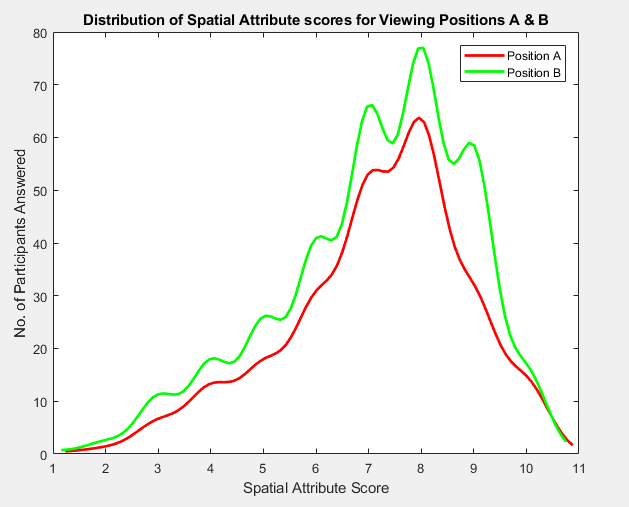
\includegraphics[width=0.5\textwidth]{images/stats/AvsB_sa_stack_all.PNG}
			\caption{Histogram showing the distribution of spatial attribute scores for viewing position A and B. This indicates that viewing position has little effect on spatial qualities in a VR environment.}
			\label{image:AvsB_dist} 
		\end{figure}

		\textbf{Conclusion}\\

		The bar chart indicates that the average spatial attribute scores are extremely close with an overall average for both being 7.1. The Two-Sample T-Test indicates that the probability of these results recurring is not unlikely ($p > \alpha (0.05)$) and therefore the results shown are not statistically significant.


	






% =========----------	[ Space left here for distraction free mode] ----------==========%









\subsection{Analysis 2: Does the choice of microphone array effect Spatial Attribute score?}
	\label{ana2}

		Breaking down the data showing in figure~\ref{image:AvsB}, figure~\ref{image:sa_allmics} shows the average spatial attribute score across all used microphone configurations. The Anderson-Darling test was used to determine that not all of the sample data (participants scores per microphone) is normally distributed. Due to non-normally distributed data the Kurskal-Wallis (K-W) ANOVA was used to determine whether any of the samples were significantly different. \\

		All groups returned a p-value greater than 0.05 other than 'Sense of Space' which returned $p = 0.0227 $. As determined in section~\ref{ana1} there is no statistical significant difference between the data from viewing positions A and B. Therefore the data was separated according to their viewing positions and another K-W test was conducted on each group. This indicated a significant difference within the group of data from viewing position B, returning $ p = 0.0035 $.

		Using MATLABs \textit{multcompare} function, a post-hoc test was conducted to determine that the sample data for two microphone arrays, OCT and Hamasaki Cube were significantly different to the sample data for the spot microphones, circled in red and blue respectively in figure~\ref{image:sa_allmics}. \\

		% NOTE: SHOULD THIS PARAGRAPH BE HERE AS IT HAS BEEN SHOWN THAT THERE IS NO STATISTICAL SIGNIFICANCE IN THE DIFFERENCES IN SCORE?
		Though little statistical significance was found between the difference microphone arrays, by analysing figure~\ref{image:sa_allmics} we can determine which microphones are overall the best choice with regards to this listening test. The two microphone arrays that showed statistical significance, the OCT and Hamasaki Cube also happen to consistently be among the top scoring microphone arrays across all spatial attributes.

		\textbf{Conclusion} \\

		For most spatial attributes, differences in mic choice is not statistically significant. However when it comes to sense of space, mixing in the microphone arrays with either the OCT or Hamasaki cube makes a significant difference relative to a pure spot mic mix. 

		\begin{figure}
			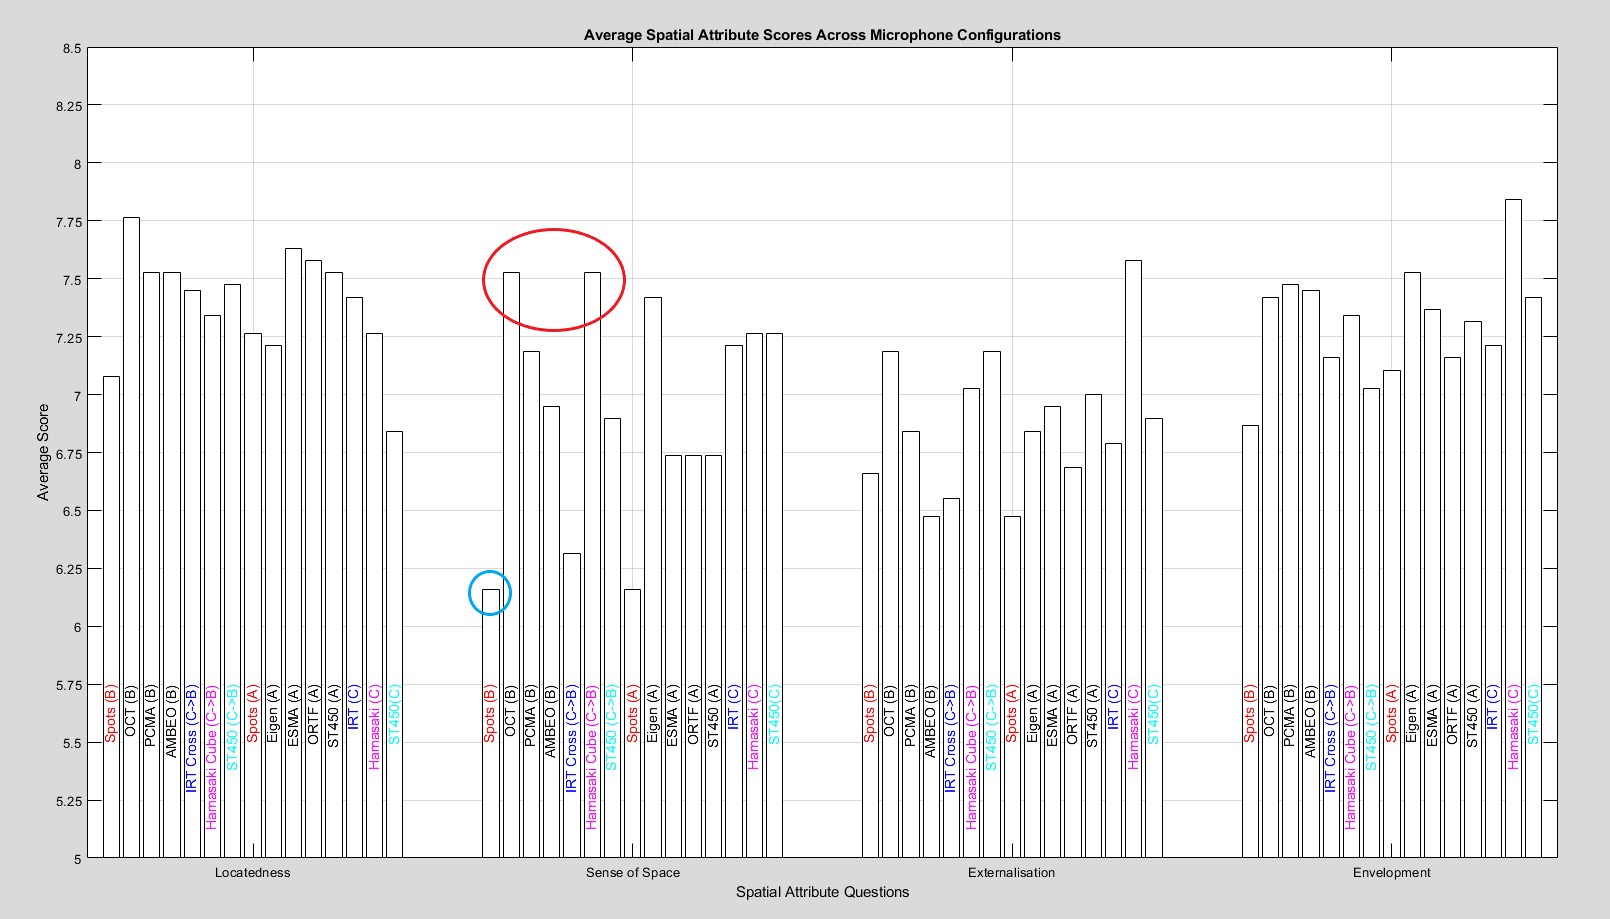
\includegraphics[width=0.5\textwidth]{images/plots/allMics_edit.PNG}
			\caption{Bar chart of the average SA score across all microphone configurations where (X) indicates the microphone location. The microphone names are displayed on their corresponding bar chart where (C->B) indicates a microphone from position C whilst viewing from B and (C) indicates a microphone from position C whilst viewing from position A}
			\label{image:sa_allmics} 
		\end{figure}


	






% =========----------	[ Space left here for distraction free mode] ----------==========%









\subsection{Analysis 3: What is the effect of using Directional or Diffuse-Field Arrays?}
	\label{ana3}

		Section~\ref{ana2} revealed no significant difference between using any of the different microphone arrays apart from when it comes to a 'Sense of Space'. However the difference was only found between using the spot mic mix against mixing the spot mics with either the OCT array or the Hamasaki Cube. As both of these microphone arrays belong to different groups (OCT is used as a directional array and the Hamasaki Cube as a diffuse field array) and were not significantly different from each other, it can also be stated that the use of directional or diffuse field arrays is also not statistically significant.

		Analysing the bar chart in figure~\ref{image:sa_allmics} however it is possible to come to some conclusions about particular microphone configurations. For example, looking at the scores for Sense of Space, the three diffuse field microphone in position C whilst viewing from position A can be said to objectively perform worse than the three of the directional microphones at position A (ESMA, ORTF, ST450). However as the Eigenmke scores higher than all of them, drawing a conclusion that one microphone type is superior would be a incorrect. A more collated visualisation of overall microphone configuration performance can be seen in figure~\ref{image:sa_allmic_avgQ}, highlighting the narrow lead of the OCT microphone configuration.

		\textbf{Conclusion}
		There appears to be no significant effect of using either a directional or diffuse-field microphone array providing that spot microphones alone are not used

		\begin{figure}
			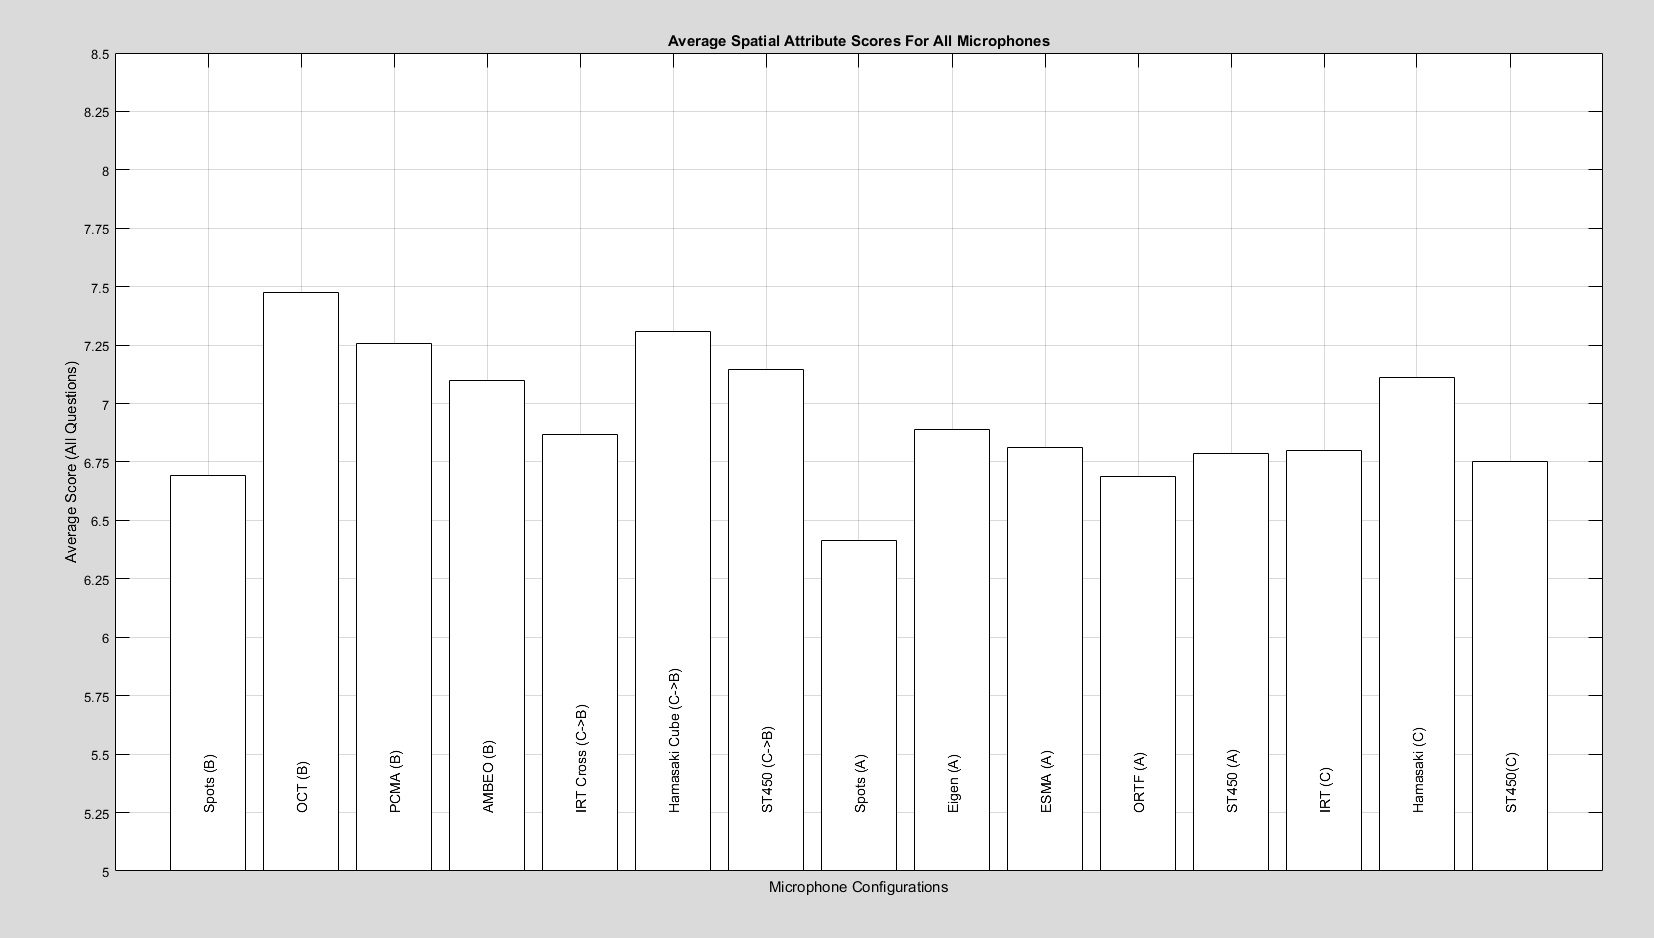
\includegraphics[width=0.5\textwidth]{{images/plots/ana3_allmics_performance.PNG}}
			\caption{}
			\label{image:sa_allmic_avgQ} 
		\end{figure}		
	






% =========----------	[ Space left here for distraction free mode] ----------==========%









\subsection{Analysis 4: Is there a difference in perception of timbre with difference viewing positions?}
\label{ana4}
		
	The effect of different viewing positions on participants perception of timbre can be assessed by comparing the data collected for microphones that were shared across both viewing positions which includes the spot microphones and microphone arrays from position C. Figure~\ref{image:ta_sharedmics} shows the percentage of participants that selected each timbral attribute for each microphone. Table~\ref{ana4:barData} presents the corresponding data showing the percentage difference between each microphone pair (each microphone at both positions) calculated by subtracting the results for microphones at position B from the same microphones at position A. For each timbral attribute, the average results column indicates whether the attribute was selected by more participants for viewing position A (positive number) or position B (negative number). By looking at the table it can be seen that across all microphones the timbral attributes 'Realistic' and 'Loud' share the trend that they were selected by an equal or greater percentage of participants for viewing position A. The timbral attribute 'Realistic' experienced the greatest variation between viewing positions with an average difference of 19\%. Though the increased frequency of participants selecting 'Loud' is only by a minor amount, it is possible that the consistency is caused simply by the fact that viewing position A is closer to the musicians thus increasing the possibility for participants to perceive the audio as 'Loud'. \\

	\begin{figure}
		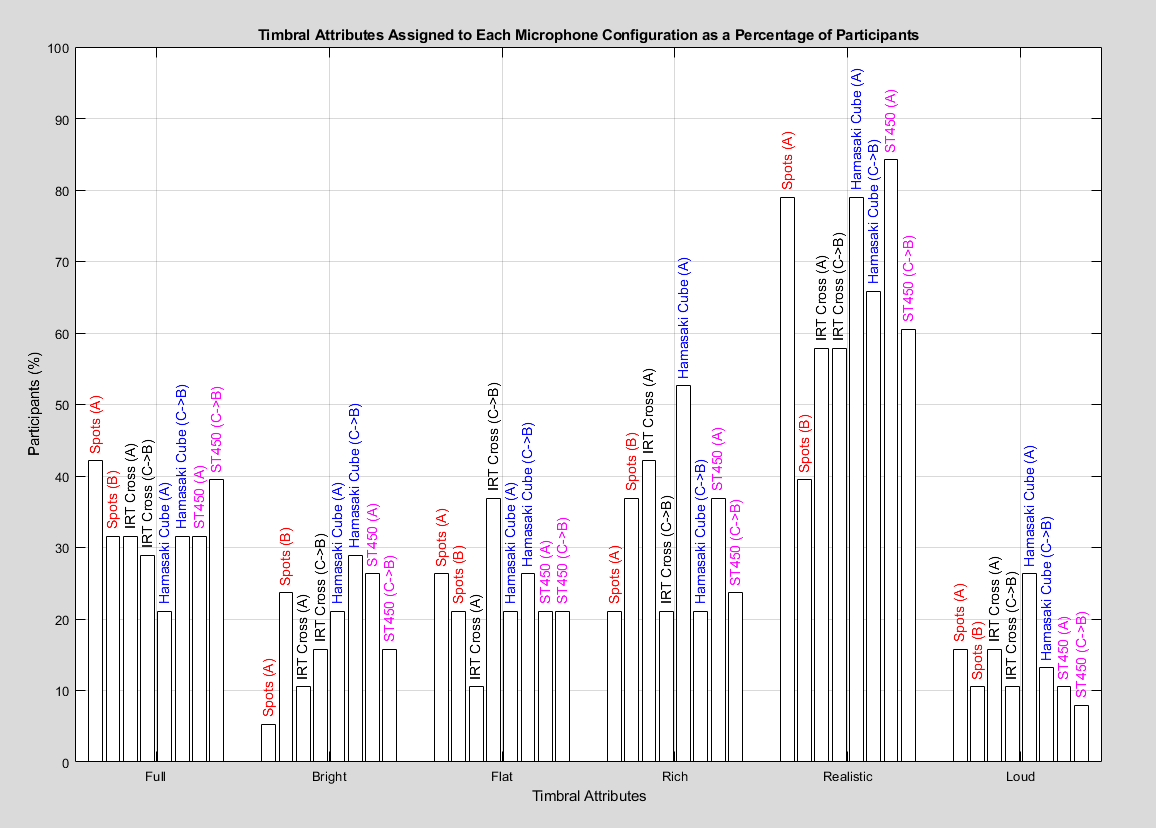
\includegraphics[width=\linewidth]{images/plots/bar_sharedMics.PNG}
		\caption{Bar chart showing the timbral attributes chosen for each microphone array shared between viewing position A and B as a percentage of participants}
		\label{image:ta_sharedmics} 
	\end{figure}	

	\begin{table}[h]
	\centering
	\resizebox{\linewidth}{!}{%
	\hspace{-15pt}
		\begin{tabular}{|>{\cen}m{15mm} |>{\cen}m{9.1mm} |>{\cen}m{9.5mm}| >{\cen}m{15mm}| *{2}{>{\cen}m{8mm}|}} \hline
		\multicolumn{1}{|>{\cen}m{12mm}|}{\multirow{2}{*}{Attributes}} & \multicolumn{4}{c|}{Microphones (\%)} & \multicolumn{1}{c|}{\multirow{2}{*}{\textbf{Averaged}}} \\ \cline{2-5}
		& Spots & IRT Cross & Hamasaki Cube & ST450 & \\ \hline
		Full & 10.53 & 2.63 & -10.53 & -7.89 & -1.32  \\ \hline
		Bright & -18.42 & -5.26 & -7.89 & 10.53 & -5.26 \\ \hline
		Flat & 5.26 & -26.32 & -5.26 & 0 & -6.58 \\\hline
		Rich & -15.79 & 21.05 & 31.59 & 13.16 & 12.5 \\ \hline
		Realistic & 39.47 & 0 & 13.16 & 23.68 & 19.08 \\ \hline
 		Loud & 5.2 & 5.2 & 13.16 & 2.63 & 6.58 \\ \hline
		\end{tabular}}
		\caption{Table showing the percentage difference between each pair of microphones calculated by $A - B$}
		\label{ana4:barData}
	\end{table}



	\textbf{Conclusion} \\

		In terms of timbre there appears to be little difference made by watching the performance from either position. The attributes effected most by changing viewing positions are a sense of whether things sounded realistic for which position A showed a preference. This increased difference however is mostly influenced by the large difference in spot microphone scores where there is a 39.5\% increase from the low 39.5\% of participants regarding the spot mics at position B to sound realistic to the 79\% of participants regarding the spot mics at position A to sound realistic. 

		It is hypothesised by the author that this is due to the unnatural lack of room acoustics heard when positioned at a distance where the sound of the room is expected to be heard. As the participant is standing much closer to the musicians at position A where the direct to reverb ratio is naturally much higher, the lack of room acoustics may be less noticeable and still be perceived as realistic. As a consequence of a lack of room acoustics present in the spot microphone mix, sound sources can be perceived more spatially isolated from one another. The unnaturalness of this is possibly less obvious when fully surrounded by the musicians as experienced at position A as this introduces an unnatural separation of the musicians for a listening experience. When viewing from position B however, as the musicians can be seen closer together, the unnatural sound source separation perceived may stand out to participants and further affect their judgement. \\


	% \begin{center}
	% \begin{table}
	% 	\begin{tabular}{r >{\centering\arraybackslash}p{30mm} c}
	% 		Attribute & Absolute Average Percentage Difference & Sway \\
	% 		Full & 7.89 & -1.32 \\
	% 		Bright & 10.53 & -5.26 \\
	% 		Flat & 9.21 & -6.58 \\
	% 		Rich & 20.39 & 12.5 \\
	% 		Realistic & 19.08 & 19.08 \\
	% 		Loud & 6.58 & 6.58 
	% 	\end{tabular}
	% 	\caption{Percentage difference}
	% 	\label{ana4:perDiff}
	% \end{table}
	% \end{center}
	






% =========----------	[ Space left here for distraction free mode] ----------==========%









\subsection{Analysis 5: Is there a correlation between spatial attribute score and selected timbral attributes?}

	Correlation coefficients were calculated for each combination of spatial attribute score against timbral attribute score. Most calculations returned weak correlations with $p > 0.05$ other than two timbral attributes specifically when comparing against the 'Envelopment' spatial attribute. Figure~\ref{image:corr_env} shows the line of best fit for all timbral attribute scores against the spatial attribute scores for 'Envelopment'. The dashed lines indicate a statistically significant correlation as found with the timbral attributes 'Full' and 'Realistic'. The graph indicates that there is a significant positive correlation between the increase in sense of 'Envelopment' in the virtual environment with the sense of the virtual environment sounding 'Realistic'.

	The data also indicates a negative correlation between participants sense of 'Envelopment' and their perception of the timbre sounding 'Full'. The reason as to why this is is not exactly clear. It could be said that participants perception of 'Full' may mean an unnatural abundance of bass frequencies which may sound unrealistic. If this is the case, as we can see from the positive correlation between a sense of 'Envelopment' and a sense of the environment sounding 'Realistic', that an unrealistic sounding environment would lead to a decrease in participants sense of 'Envelopment'. 

	\textbf{Conclusion}

	The only spatial attribute to show a significant correlation with timbral attribute data is 'Sense of Space' with a positive correlation for a perception of the mix sounding 'Realistic' and a negative correlation for the perception of the mix sounding 'Full'.

	\begin{figure}
		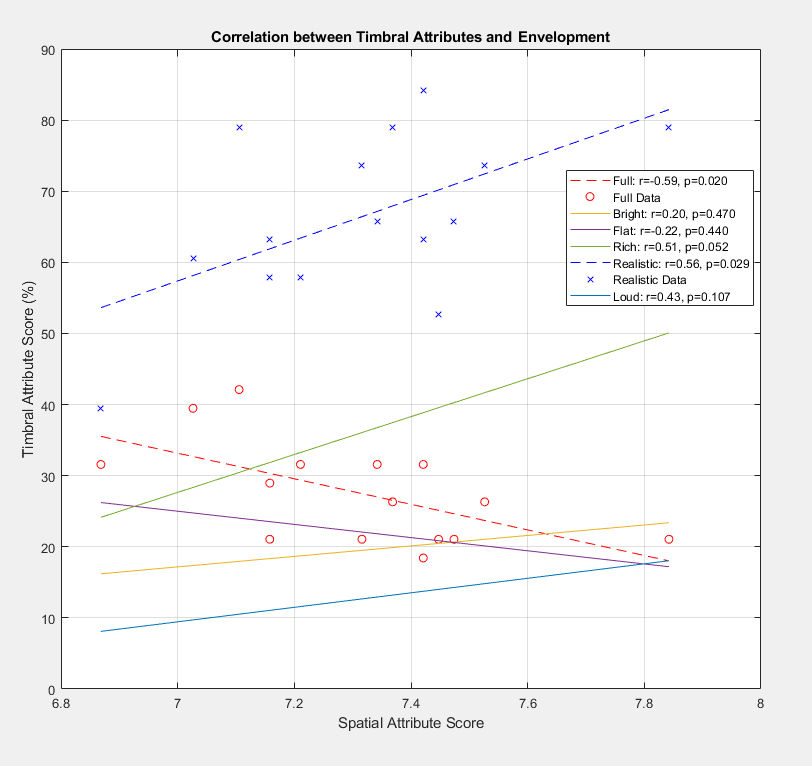
\includegraphics[width=\linewidth]{images/plots/sa_ta_corr_env.PNG}
		\caption{Graph showing correlations between Timbral Attribute and Envelopment scores where dashed lines indicate a statistically significant correlation for which their individual data points have also been plotted.}
		\label{image:corr_env} 
	\end{figure}		

	






% =========----------	[ Space left here for distraction free mode] ----------==========%









\subsection{Analysis 6: Enjoyment Factor}

	As VR is designed to entertain, participants were asked to rate on a scale of 1-10 how much they felt they enjoyed the experience. Figure~\ref{image:enjoyment} shows the line of best fit for everage enjoyment rating againt average spatial attribute for each microphone for both viewing position A and B.
	

	\begin{figure}
		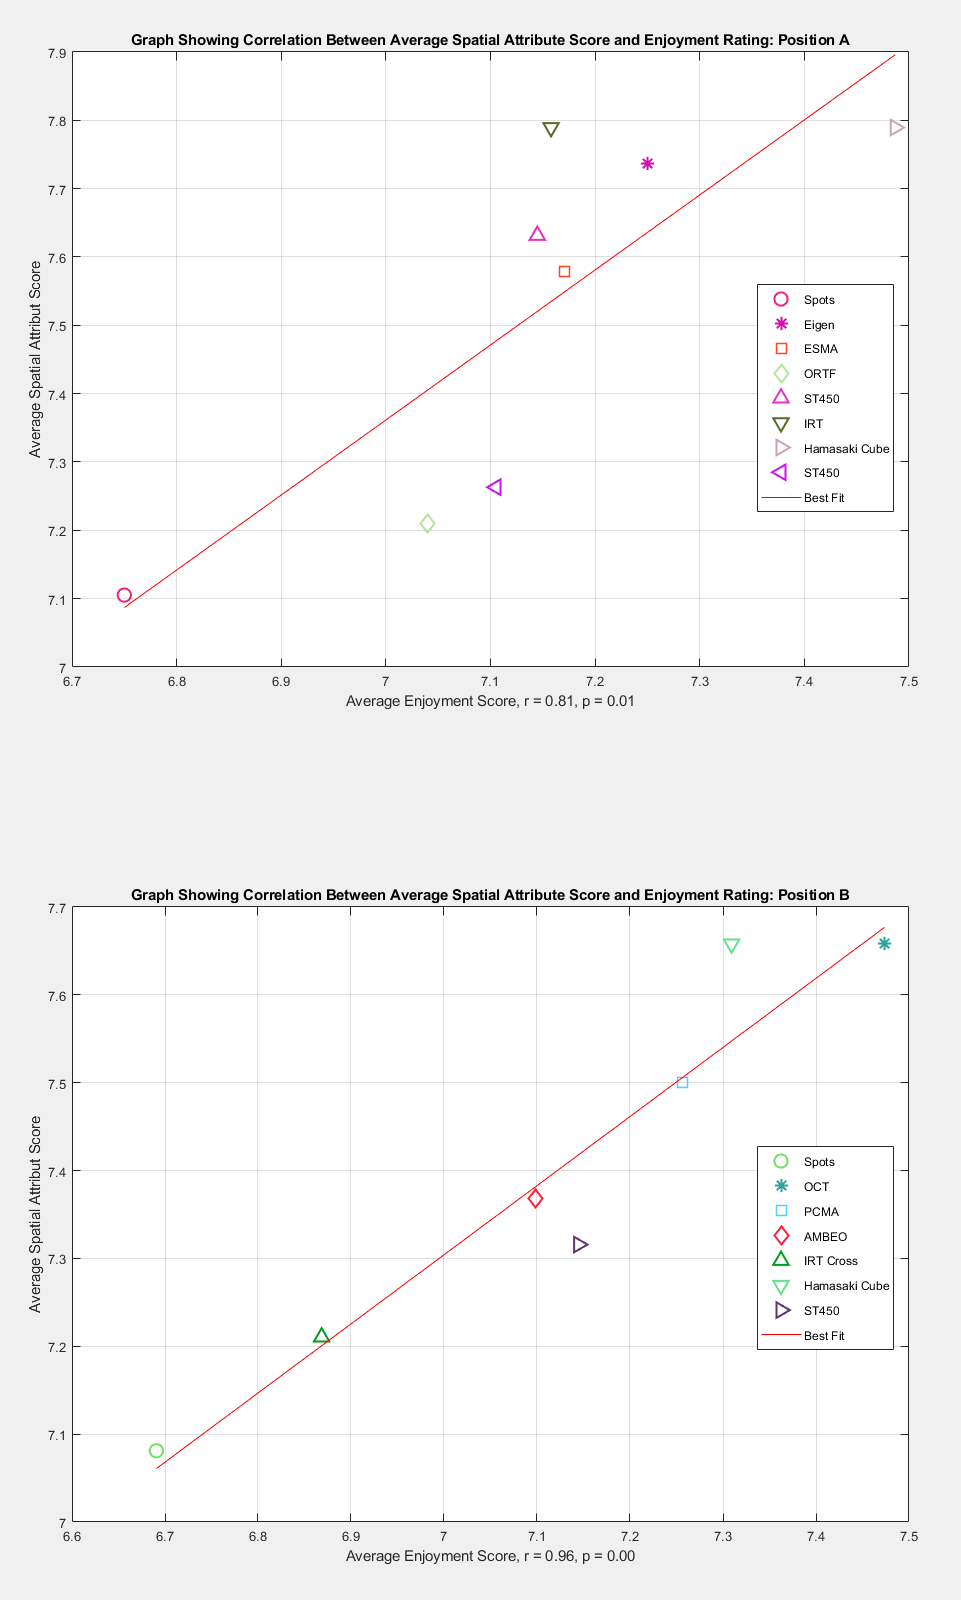
\includegraphics[width=0.5\textwidth]{images/plots/enjoyment_corr_V1.PNG}
		\caption{Two graphs showing a positive correlation between enjoyment rating and spatial attribute scores for viewing positions A (Top) and B (Bottom).}
		\label{image:enjoyment} 
	\end{figure}		


	\section{Analysis Summary}
		% Summarise the results

		The analysis of the data can be summarised as follows:

		Analysis 1: Viewing the performance from position A (360\textdegree perspective) or position B (180\textdegree perspective) has no significant difference on participants spatial attribute scores.

		Analysis 2: OCT and Hamasaki Cube were found to be statistically significant with regards to the spatial attribute 'Sense of Space'. This can be seen as a significantly poor performance from the spot microphones at viewing position B. Though little statistical significance was found between the different microphone arrays, by analysing figure~\ref{image:sa_allmics} in section~\ref{ana2} we can determine which microphones are overall the best choice with regards to this listening test. The two microphone arrays that showed statistical significance, the OCT and Hamasaki Cube also happen to consistently be among the top scoring microphone arrays across all spatial attributes.

		Analysis 3: There appears to be no significant difference between using either a direct or diffuse-field microphone array so long as spot microphones alone are not used.

		Analysis 4: Timbre itself seems to be unaffected by the viewing positions. However participants perception of the mix sounding 'realistic' and 'loud' appears to be the most affected with a higher score for viewing position A. It is hypothesised that this is due to the unnatural room acoustic and sound source separation caused when listening to the spot mic mix that skews the result this way.

		Analysis 5: A statistically significant positive correlation was found between sense of space and the perception of the mix being 'realistic'. A significant negative correlation was also found between sense of space and the perception of the timbre sounding 'Full'.



\bibliographystyle{aes2e}
\bibliography{aes2e}

\end{document}
